\section{\textbf{Simulation study}}

We explore the utility of AME as an inferential tool for dyadic analysis via a simulation exercise.\footnote{Alternative network based approaches for dyadic data are exponential random graph models (ERGMs) and the related stochastic actor oriented model (SAOM). While both these models have led to numerous contributions to a variety of literatures, the applicability of these approaches may be limited to certain types of networks and individual level characteristics. Specifically, \citet{block:etal:2017} note that these types of  models may not be appropriate in situations where network and behavioral data depend on unobserved latent variables, which is explicitly the focus of our analysis here.} Most scholars working with dyadic data are primarily concerned with understanding the effect of a particular independent variable on a dyadic dependent variable. The goal of our simulation is to assess how well AME can provide unbiased and well-calibrated estimates of regression coefficients in the presence of unobserved dependencies, specifically, homophily. As discussed in the previous section, homophily is the idea that actors are more likely to have a tie if they have similar values on a particular variable, and in networks the presence of homophily can lead to third order dependencies such as transitivity. Homophily can be operationalized by creating a dyadic covariate via the multiplication of a nodal covariate with its transpose. For example, if the nodal covariate was a binary indicator for democracy, multiplying it by its transpose would give us a dyadic covariate that represents whether any dyad is jointly democratic or not.\footnote{This process of operationalizing homophily is equivalent to the `nodematch` function in the `ergm` and `latentnet` packages. There are many other options of operationalizing homophily including calculating the difference in scores that a pair of actors may have on a particular nodal variable.}

Assume that the true data-generating process for a binary variable, $Y$, is given by:

\begin{align}
	Z_{i,j} &=  \mu + \beta X_{i,j} + \gamma W_{i,j} + \epsilon_{i,j}, \; \epsilon \sim normal(0,1) \nonumber \\
	Y_{i,j} &= I(Z_{i,j} > 0)
	\label{eqn:sim}
\end{align}

$X_{i,j} = x \times x^{T}$, where $x$ is a nodal covariate that is drawn from a standard normal distribution. Similarly,  $W_{i,j} = w \times w^{T}$, where $w$ is also a nodal covariate that is independently drawn from a standard normal distribution. We generate our binary dependent variable, $Y$, within a probit framework with $Z$ serving as the latent variable. $X$ and $W$ are both dyadic covariates that are a part of the data-generating process for $Y$, but $W$ is not observed. We compare inference for $\mu$ and $\beta$---the latter parameter would be of primary concern for applied scholars---using three models:

\begin{itemize}
	\item the ``standard'' international relations approach estimated through a generalized linear model;\footnote{Specifically, here we are just regressing $Y$ on $X$ assuming independent errors.}
	\item the AME approach outlined in the previous section with a unidimensional latent factor space ($K=1$);\footnote{Results with higher values of $K$ are similar.}
	\item and an ``oracle'' regression model that assumes we have measured all sources of dependencies and thus includes both $x_{i,j}$ and $w_{i,j}$.
\end{itemize}

The first model corresponds to the ``standard'' approach in which little is explicitly done to account for dependencies in dyadic data. In the second model, we use the AME framework described in the previous section. For both the first and second models, we are simply estimating a linear model of $X$ on $Y$, and assessing the extent to which inference on the regression parameters are complicated by the presence of unobserved dependencies, $W$. In the last model, we provide an illustration of the ideal case in which we have observed and measured $W$ and include it in our specification for $Y$. The oracle case provides an important benchmark for the standard and AME approaches.

For the simulation we set the true value of $\mu$ (the intercept term) to -2 and $\beta$ (the effect of $X$ on $Y$) to 1.\footnote{The value of $\gamma$ is also set to 1, which corresponds to an example where the $W$ character is associated with homophily.} We conduct two sets of simulations, one in which the number of actors in the network is set to 50 and the other at 100. In total, we run 1,000 simulations where we begin by simulating $Y$ from the specification given in Equation~\ref{eqn:sim} and then for each simulated $Y$ we estimate a standard, AME, and oracle model.

We first compare the performance of the models in terms of how well they estimate the true values of $\mu$ and $\beta$ in Figure~\ref{fig:ameBias}. The panels on the left show the results for when the number of actors is set to 50 and on the  right for 100 actors. The top pair of panels represents the estimates for $\mu$ while the bottom pair do the same for $\beta$. In each case, we find that the estimates for $\mu$ and $\beta$ produced by the standard approach are notably off from their true values. On the other hand, the AME model performs just as well as the oracle at estimating the true parameter values.

\begin{figure}
	\centering
	\caption{Regression parameter estimates for the standard, AME, and oracle models from 1,000 simulations. Summary statistics are presented through a traditional box plot, and the estimates from each simulation are visualized as well as points.}
	\label{fig:ameBias}
	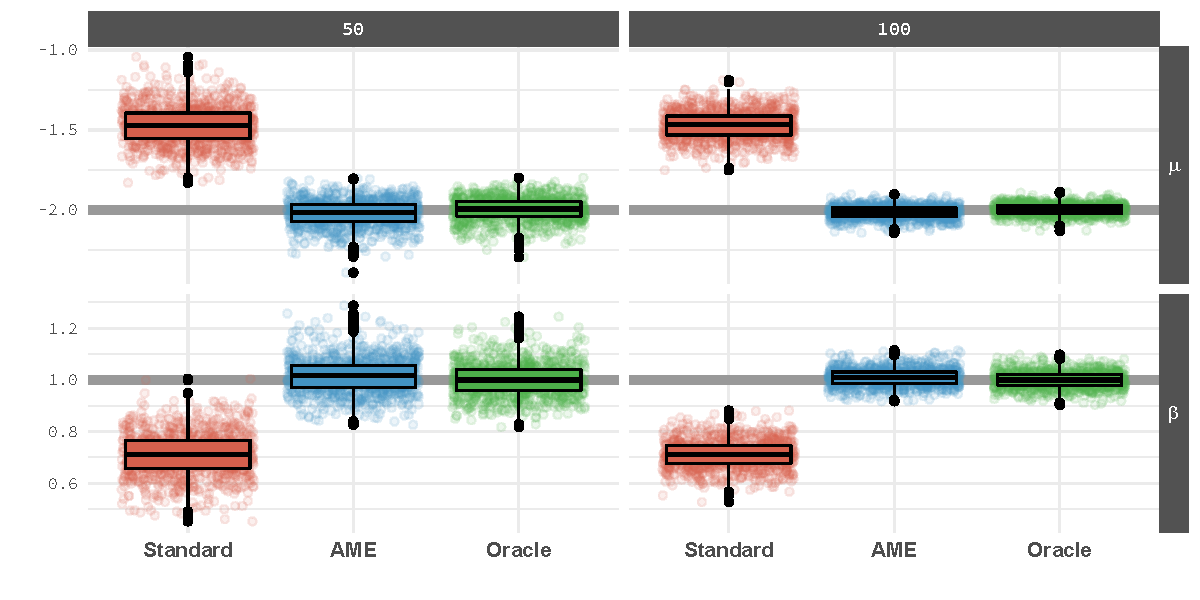
\includegraphics[width=1\textwidth]{graphics/figure3.pdf} \\
\end{figure}

Next, we estimate the 95\% credible interval for the three models in each of the simulations and estimate the proportion of times that the true value fell within those intervals. The results are summarized in Figure~\ref{fig:ameCalib}, and again we see that the AME approach performs as well as the oracle, while the standard approach performs poorly by comparison. The implication of the results presented in Figures~\ref{fig:ameBias} and ~\ref{fig:ameCalib} is that standard approaches can often fail at estimating parameter values and conducting inferential tasks in the presence of unobserved dependencies. The AME approach by comparison can be used as a tool for scholars working with dyadic data to still estimate the true effects of their main variables of interest, while accounting for dependencies that do often emerge in dyadic data.

\begin{figure}
	\centering
	\caption{Proportion of times the true value fell within the estimated 95\% confidence interval for the standard, AME, and oracle models from 1,000 simulations.}
	\label{fig:ameCalib}
	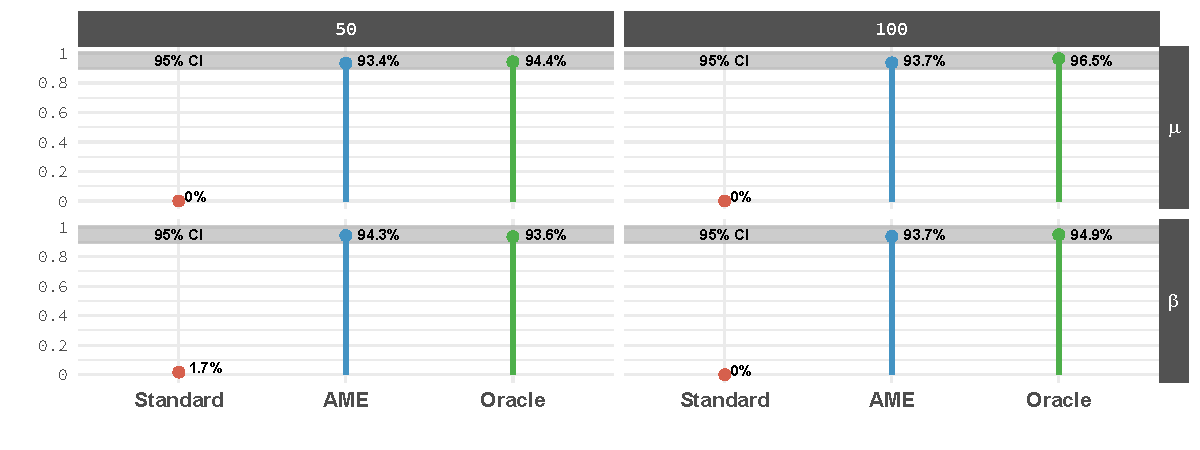
\includegraphics[width=1\textwidth]{graphics/figure4.pdf} \\
\end{figure}

Moreover, the AME approach allows scholars to better understand what parameters their model may be missing. In the case of the simulation here, $W$ is set as an unobserved dyadic covariate that has a homophilous effect on $Y$. The effect of $W$ is homophilous within this framework because it is a dyadic attribute involving $i$ and $j$ that positively affects the degree to which actors interact with one another, i.e., $y_{ij}$. This type of unobserved dependency will be captured through the multiplicative effects portion of the model, $\mathbf{U}^{\top} \mathbf{D} \mathbf{V}$. To estimate how well the model performs, we recover the multiplicative effects term for each simulation and calculate the correlation between it and the unobserved dependency, $W$.\footnote{Specifically, since both the multiplicative effects term and $W$ are continuous dyadic variables, we calculate the Pearson correlation coefficient.} We visualize the distribution of the correlations from each of the 1,000 simulations in Figure~\ref{fig:ameCorr} for the case where the number of actors is set to 100 (top pair of panels) and 50. Additionally, we calculate the median across the correlations and display the result using a vertical line. For both $n=50$ and $n=100$, we find that the multiplicative effects perform very well in capturing the unobserved dependency, which indicates that the AME does not simply capture noise but also works as a tool to estimate unobserved structure.

\begin{figure}
	\centering
	\caption{Distribution of correlation between missing variable and multiplicative random effect in AME across the 1,000 simulations. Vertical line through the distribution represents the median value across the simulations.}
	\label{fig:ameCorr}
	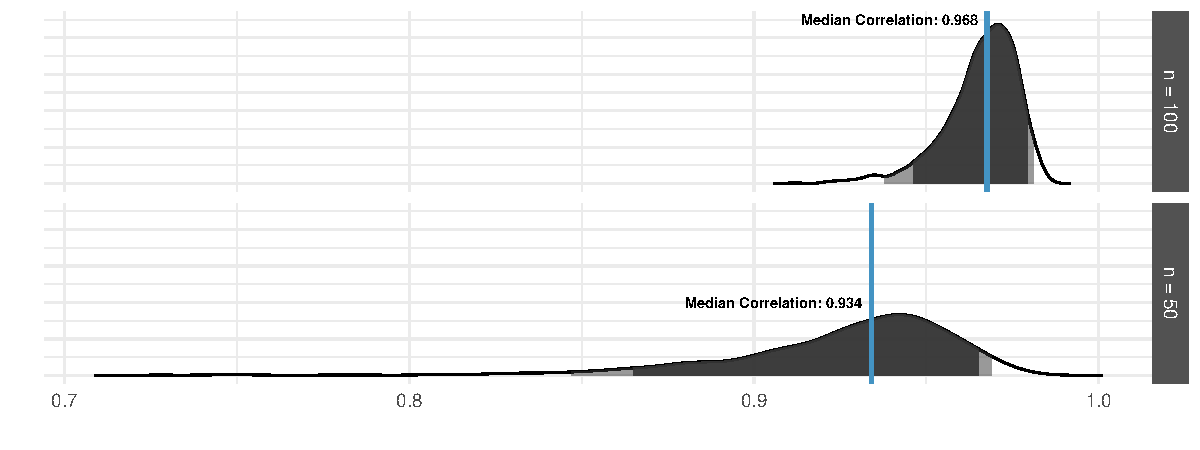
\includegraphics[width=1\textwidth]{graphics/figure5.pdf} \\
\end{figure}

The simulation shows that beyond obtaining less biased and better-calibrated parameter estimates, a key benefit of the AME framework is to directly estimate unobserved dependencies through the random effects structure of the model. Scholars can use this framework in an iterative fashion: beginning with an estimated model, they can then empirically study the structure of the random effects to assess whether there are unobserved covariates that they want to include in their model. Importantly, this simulation underscores how a careful consideration of a systems' interconnectedness, both through theoretical approaches and empirical models, can result in more precise estimates of direct and indirect effects across the system.

%older: This simulation also demonstrates that the AME model can help conduct inference and estimate the true effect of independent variables that scholars operationalize to test theoretical propositions.
